\documentclass[12pt]{article}
\usepackage{graphicx}
%\documentclass[journal,12pt,twocolumn]{IEEEtran}
\usepackage[none]{hyphenat}
\usepackage{graphicx}
\usepackage{listings}
\usepackage[english]{babel}
\usepackage{graphicx}
\usepackage{caption}
\usepackage[parfill]{parskip}
\usepackage{hyperref}
\usepackage{booktabs}
%\usepackage{setspace}\doublespacing\pagestyle{plain}
\def\inputGnumericTable{}
\usepackage{color}                                            %%
    \usepackage{array}                                            %%
    \usepackage{longtable}                                        %%
    \usepackage{calc}                                             %%
    \usepackage{multirow}                                         %%
    \usepackage{hhline}                                           %%
    \usepackage{ifthen}
\usepackage{array}
\usepackage{amsmath}   % for having text in math mode
\usepackage{parallel,enumitem}
\usepackage{listings}
\lstset{
language=tex,
frame=single, 
breaklines=true
}
  
%Following 2 lines were added to remove the blank page at the beginning
\usepackage{atbegshi}% http://ctan.org/pkg/atbegshi
\AtBeginDocument{\AtBeginShipoutNext{\AtBeginShipoutDiscard}}
%
%New macro definitions
\newcommand{\mydet}[1]{\ensuremath{\begin{vmatrix}#1\end{vmatrix}}}
\providecommand{\brak}[1]{\ensuremath{\left(#1\right)}}
\providecommand{\abs}[1]{\left\vert#1\right\vert}
\providecommand{\norm}[1]{\left\lVert#1\right\rVert}
\newcommand{\solution}{\noindent \textbf{Solution: }}
\newcommand{\myvec}[1]{\ensuremath{\begin{pmatrix}#1\end{pmatrix}}}
\let\vec\mathbf
\begin{document}
\begin{center}
\title{\textbf{Parallel Lines}}
\date{\vspace{-5ex}} %Not to print date automatically
\maketitle
\end{center}
\setcounter{page}{1}
\section*{11$^{th}$ Maths - Chapter 10}
This is Problem-6 from Exercise 10.3
\begin{enumerate}
	\item Find the distance between parallel lines 
	
(i) 15x+8y-34=0 and  15x+8y+31=0 \\
(ii) l(x+y)+p=0 and  l(x+y)-r=0
\	
\item solution for problem 1
\\
Given line is 
\begin{align}
	15x+8y-34=0\text{ and }15x+8y+31=0
\end{align}
this equation can be expressed as 
\begin{align}
	\vec{n}^{\top}\vec{x}=c_1\\	
	\vec{n}^{\top}\vec{x}=c_2	
\end{align}
\begin{align}
\text{ where }
\vec{n}&=\myvec{15\\8},c_1=-34, c_2= 31\\
& \myvec{15&8}\vec{x}=-34\\ 
& \myvec{15&8}\vec{x}=31\\
\end{align} 
distance between parallel lines 
\begin{align}
d&=\frac{\abs{c_1-c_2}}{\norm{n}}\\
&=\frac{\abs{-34-31}}{\sqrt{289}}\\
&=\frac{65}{17}
\end{align}
\begin{figure}[h!]
\begin{center}
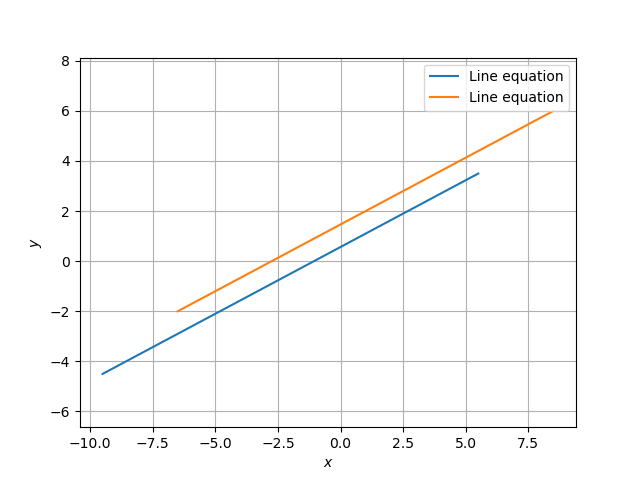
\includegraphics[width=\columnwidth]{para.png}
\end{center}
\caption{}
\label{fig:Fig1}
\end{figure}
	\item solution for problem 2
	\\
Given line is 
\begin{align}
l(x+y)+p=0\text{ and }l(x+y)-r=0
\end{align}
this equation can be expressed as 
\begin{align}
\vec{n}^{\top}\vec{x}=c_1\\
\vec{n}^{\top}\vec{x}=c_2
\end{align}
\begin{align}
\text{ where }
\vec{n}& = \myvec{l\\l},c_1=p,c_2=-r\\
& =\myvec{l&l}\vec{x}=p\\ 
& =\myvec{l&l}\vec{x}=-r		
\end{align}
distance between parallel lines 
\begin{align}
d&=\frac{\abs{p-(-r)}}{\sqrt{l^{2}}}\\
&=\frac{\abs{p+r}}{l\sqrt{2}}
\end{align}	
The distance between parallel lines 
is shown in figure \eqref{fig:Fig2} with normal vector as 
\begin{align*}
\vec{n} =\myvec{8\\8} \text{ and }c_1=16,c_2=-16
\end{align*}
\begin{figure}[h!]
\begin{center}
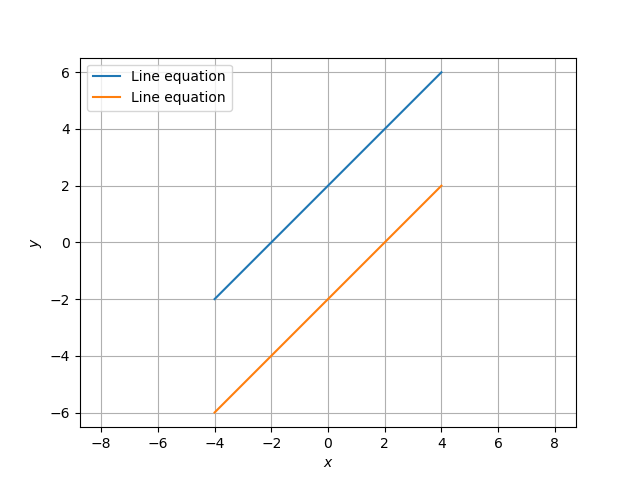
\includegraphics[width=\columnwidth]{para1.png}
\end{center}
\caption{}
\label{fig:Fig2}
\end{figure}
\end{enumerate}
\end{document}